% Preamble
\documentclass[11pt]{article}

% Packages
%\usepackage{a4wide}
\usepackage[a4paper]{geometry}
\usepackage[english]{babel}
\usepackage[utf8]{inputenc}
\usepackage{xargs}                      % Use more than one optional parameter in a new commands
\usepackage[pdftex,dvipsnames]{xcolor}  % Coloured text etc.
\usepackage{graphicx} % Images etc.
\usepackage[hidelinks]{hyperref} % Makes citations clickable
\usepackage{amssymb}
\usepackage{amsmath}
\usepackage{mathtools} % e.g ":="

\usepackage[colorinlistoftodos,prependcaption,textsize=tiny]{todonotes}

\newcommandx{\unsure}[2][1=]{\todo[linecolor=orange,backgroundcolor=orange!25,bordercolor=orange,#1]{#2}}
\newcommandx{\Todo}[2][1=]{\todo[linecolor=yellow,backgroundcolor=yellow!25,bordercolor=yellow,#1]{#2}}

\renewcommand{\baselinestretch}{1.15} % line distance

\author{Nikolas Klug \\ Universität Augsburg}
\date{\today}
\title{To be determined}


\begin{document}
	\maketitle
	\newpage
	\begin{abstract}
		This is the abstract.
	\end{abstract}
	\newpage
	\tableofcontents
	\newpage
	\section{Introduction}
	\section{Network architecture}
	\section{Data}
	Assumptions:
	\begin{itemize}
		\item All 2d data can be scaled in a way that a norm limb is of length 0.1. 
		Problems with correct camera distance, see section \ref{sec:z-shift-error}
	\end{itemize}
	\subsection{Evaluation Metrics}
	\subsubsection{Protocol 2}\label{sec:protocol2}
	%	
\section{Protocols}
\subsection{Protocol 1}
	\begin{itemize}
		\item Training: S1, S5, S6, S7, S8, S9 (commonly used, e.g. in \cite{chen17})
		\begin{itemize}
			\item \cite{drover18} do not use S9.
			\item The available code suggests that not every pose is used, but only such where at least one joint has moved by 40mm with respect to the former frame.
		\end{itemize} 			
		\item Evaluation: S11
		\begin{itemize}
			\item \cite{sun17} use every 64th frame (and also the code suggests this). If they only use the available code this would mean they use all four cameras.
			\item \cite{drover18} use ground truth 2d points for testing (might be the same as \cite{sun17})
			\item \cite{moreno-noguer16} use every 64th frame of the frontal view for testing
		\end{itemize}

		\item Error: \begin{itemize}
			\item \cite{drover18} use Mean per Joint Position Error (MPJPE) with scaling and rigid alignment to the ground truth skeleton (they don't mention which exactly)
			\item \cite{sun17} also use MPJPE after rigid alignment using Procrustes Analysis
			\item \cite{yasin16} use the MPJPE after alignment to the ground truth skeleton by a rigid transformation (they don't mention which exactly)
			\item \cite{kostrikov14} align the poses by a rigid transformation using \emph{least squares} before computing the MPJPE error
			\item \cite{tome17} perform a similarity transformation using a Procrustes Analysis
		\end{itemize}
		
	\end{itemize}
\subsection{Protocol 2}
	\begin{itemize}
		\item Training: S1, S5, S6, S7, S8
		\begin{itemize}
			\item Similar to protocol 1 the code suggests that not every pose is used, but only such where at least one joint has moved by 40mm with respect to the former frame.
			\item \cite{bogo16} evaluate on five different action sequences captured from the frontal camera
			\item \cite{tekin16, tekin17} use all camera views for training
		\end{itemize}
		\item Evaluation: S9, S11 
		\begin{itemize}
			\item \cite{sun17} use every 64th frame
			\item \cite{tekin16, tekin17} use all camera views for testing
			\item \cite{bogo16} evaluate on five different action sequences captured from the frontal camera
			\item \cite{moreno-noguer16} say they use all images for testing (whatever this means) 
		\end{itemize}
		\item Error: \begin{itemize}
			\item \cite{sun17} use MPJPE apparently without any alignment and scaling
			\item \cite{martinez17} align the root (central hip), they do not mention any scaling
			\item \cite{tome17} do not mention any alignment
			\item \cite{zhou18} scale the output such that the mean limb length is identical to the average value of all training subjects and align the root locations. Procrustes Analysis is not allowed.
			\item \cite{bogo16} apply a similarity transformation to align the reconstructed 3D joints via the Procrustes analysis on every frame
			\item \cite{zhou16} align the root locations and scale the output such that the mean limb length is identical to the average value of all training subjects. Procrustes alignment is not allowed.
			\item it seems that \cite{tekin16} also align the root nodes
			\item \cite{tekin17} use a Procrustes transformation before measuring the MPJPE
			\item \cite{pavlakos17} align the root joints
		\end{itemize}
	\end{itemize}

\subsection{Miscellaneous}
\begin{itemize}
	\item \cite{jahangiri17} evaluate using all subjects after a similarity transformation obtained by Procrustes alignment
\end{itemize}

\section{Questions and Problems}
\begin{itemize}
	\item It is sometimes not clear which 2d poses are used for testing.
	\item The transformations applied before calculating the error are not consistent within the protocols.
\end{itemize}


\section{Our approach}
	\subsection{Protocol 1}
		\begin{itemize}
			\item Training subjects: S1, S5, S6, S7, S8, S9
			\item Testing/Evaluation subjects: S11
			\item For now we train on all frames available, \emph{not} such where at least one joint has moved by 40mm
			\item For evaluation every 64th frame available for the according subjects is used
			\item Error metric: MPJPE
			\item Before calculating the error, the poses are transformed using a Procrustes Transformation and the root nodes are aligned
		\end{itemize}
	\subsection{Protocol 2}
		\begin{itemize}
			\item Training subjects: S1, S5, S6, S7, S8
			\item Testing/Evaluation subjects: S9, S11
			\item For now we train on all frames available, \emph{not} such where at least one joint has moved by 40mm
			\item For evaluation every 64th frame available for the according subjects is used
			\item Error metric: MPJPE
			\item Before calculating the error, the root nodes are aligned and the pose is scaled such that the mean limb length is identical to the average value of all training subjects
		\end{itemize}
 
	\subsection{Results for data}
	\subsection{Different errors for different sets of joints}
		Using only 15 joints yields a much lower MPJPE than using 32 joints. Reasons: ...	
		From now on all numbers are calculated for 15 joint poses.
	\section{Part 1: MPJPE increase when shifting}
	
	Possible deviations of the assumptions about the three dimensional poses and how they are projected onto the image plane: Deviation in x and y direction, deviation in z direction, different focal length.
	
	We regard the system as a black box that takes a normalized set of two dimensional points as input and outputs the depths (the z coordinates) of the input points which then can be reprojected into three dimensional space.
	\subsection{Shifting along one image plane axis}
	\Todo{Add introduction to nomenclature and notation.}
	\label{sec:x-shift-error}
	\subsubsection{Theoretical analysis}
	\Todo{Properly define the pose and the camera.}
	Let $P_i=(x_i, y_i, z_i) \in \mathbb{R}^3$ and $f$ the focal length of a camera which is located at the origin along the x-y-plane and looks at $(0, 0, z)$, the location of the root joint. 
	Assume $P_i$ is shifted by $dx$ along the x axis.
	The x coordinate of the projected point on the image plane is
	\begin{equation}
		x_i^\mathrm{P} = f \frac{x_i + dx}{z_i} = f \frac{x_i}{z_i} + f \frac{dx}{z_i}\ .
	\end{equation}
	Subsequently all projected points are shifted along the x axis such that the root node which is located at $(0, 0, z)$ is in the origin of the image plane. That means:
	\begin{equation}
		\widetilde{x}_i^\mathrm{P} = f \frac{x_i}{z_i} + f \frac{dx}{z_i} - f \frac{dx}{z} 
		= f \frac{x_i}{z_i} + f dx (\frac{1}{z_i} - \frac{1}{z})
		= x_i^\mathrm{P} + f dx (\frac{1}{z_i} - \frac{1}{z})\ .
	\end{equation}
	After the system estimated the depth $\widetilde{z}_i$ of the point, it is reprojected into three dimensions. The resulting x coordinate is 
	\begin{equation}
		\widetilde{x}_i^\mathrm{R} = \frac{\widetilde{x}_i^\mathrm{P}}{f} \cdot \widetilde{z}_i
		= x_i \frac{\widetilde{z}_i}{z_i} + dx (\frac{1}{z_i} - \frac{1}{z}) \widetilde{z}_i
	\end{equation}
	The euclidean distance of the reprojected point to the original point is given by
	\begin{equation}
	\label{eq:delta-d}
		\Delta d_i = \left \| 
		\begin{pmatrix}
			\widetilde{x}_i^R - x_i \\
			\widetilde{z}_i - z_i
		\end{pmatrix}
		\right \|_2
	\end{equation}
	This expression takes on its minimum when 
	\begin{equation}
		\label{eq:minimum-distance}
		f(\widetilde{z}_i) = \left ( \widetilde{z}_i \cdot \left( \frac{x_i}{z_i} + dx \left( \frac{1}{z_i} - \frac{1}{z} \right) \right ) - x_i \right)^2 + ( \widetilde{z}_i - z_i ) ^2
	\end{equation}
	is minimal. 
	Substituting $a = \left( \frac{x_i}{z_i} + dx \left( \frac{1}{z_i} - \frac{1}{z} \right) \right )$ makes the equation more readable. 
	In order to obtain the optimal value for $\widetilde{z}_i$, \eqref{eq:minimum-distance} is differentiated by $\widetilde{z}_i$:
	\begin{equation}
		f'(\widetilde{z}_i) = 2 \cdot (\widetilde{z}_i a^2 - a x_i + \widetilde{z}_i - z_i)
	\end{equation}
	Setting this equal to zero gives
	\begin{align*}
		0 &= f'(\widetilde{z}_i) \\
		\Leftrightarrow \widetilde{z}_i & = \frac{a x_i + z_i}{1 + a^2} \ .
	\end{align*}
	Substituting this into \eqref{eq:delta-d} again yields a total minimal error of 
	\begin{equation}
		\label{eq:minimum-delta-d}
		\Delta d_i = \sqrt{\frac{(a z_i - x_i)^2}{a^2 + 1}}\
		= dx (1 -  \frac{z_i}{z}) \sqrt{\frac{1}{a^2 + 1}} .
	\end{equation}
	The MPJPE $\Delta d$ for a pose can then be calculated as the mean of all $\Delta d_i$s.
	
	\subsubsection{Experimental results}
		In practice, the observable error has the same approximate shape of this function, but is much smaller than the theoretical results.
		The reason for this is the scaling that is applied to the inferred poses during the evaluation of Protocol 2 (section \ref{sec:protocol2}).
		\unsure{Validate if this is really the case. Also see in what way it is proportional.}
		It appears that the average limb length of the inferred shifted poses is increasing monotonously with increasing offset $dx$.
		That means the poses are downsized by a factor $\alpha$ in all dimensions. 
		\Todo{Explain why} Therefore the actual error is $\Delta d' = \alpha \cdot \Delta d$.
		
		\begin{figure}[ht]
			\centering
			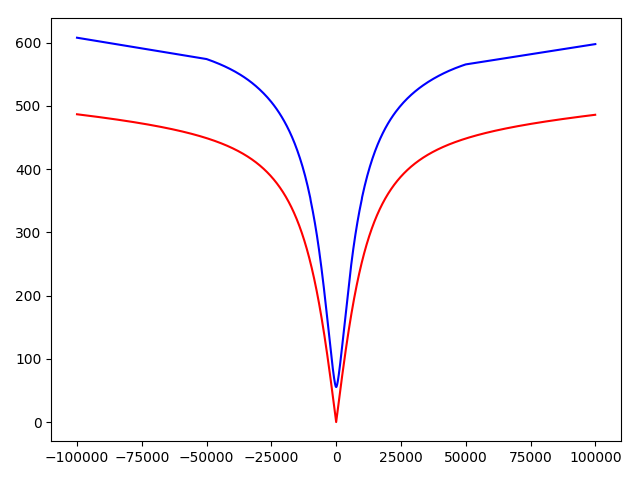
\includegraphics[scale=0.5]{images/x_shift_error.png}
			\caption{Plot of theoretical (red) and observed (blue) MPJPEs for different values of $dx$. 
				The theoretical errors are obtained by calculating the mean of the per pose errors $\alpha \Delta d$ for the evaluation data.}
			\Todo[inline]{Add axes titles, use proper image}
			\label{fig:x-shift-error}
		\end{figure}
	
		It is noticeable that the performance of the network is not worse than the theoretical results by a constant offset.
		For small deviations along the x axis the network seems to be able to compensate the error introduced by shifting.
		As $dx$ increases, so does the offset between the observed and the theoretical results until it seems to converge to a constant.
		This motivates adjusting not only how the inferred points are reprojected into three dimensions but also the input the network receives.
		This will be discussed further in section \ref{sec:network-adjusting}.
		
	\subsection{Shifting along the z axis}
	\label{sec:z-shift-error}
	\subsubsection{Theoretical analysis}
	Again consider a point $P_i=(x_i, y_i, z_i) \in \mathbb{R}^3$. Assume that $P_i$ is shifted by $dz$ along the z axis.
	The x coordinate of the projected point on the image plane is
	\begin{equation}
		x_i^\mathrm{P} = f \frac{x_i}{z_i + dz}
	\end{equation}
	The projected points are now scaled in a way that they have the same (arbitrary) scale.  Let $\alpha$ be the scale of the set of the original projected points and $\beta$ the one of the set of shifted projected points. The scaled projected point is given by
	
	\begin{equation}
			\widetilde{x}_i^\mathrm{P} = x_i^\mathrm{P} \cdot \frac{\alpha}{\beta} 
			= f \frac{x_i}{z_i + dz}\cdot \frac{\alpha}{\beta} 
	\end{equation}
	After the system estimates the depth $\widetilde{z}_i$ of each point, they are reprojected into 3 dimensional space.
	The reprojected points are given by
	\begin{equation}
		\widetilde{x}_i^\mathrm{R} = \frac{\widetilde{x}_i^\mathrm{P}}{f} \cdot \widetilde{z}_i
		= \frac{x_i}{z_i + dz}\cdot \frac{\alpha}{\beta}  \cdot \widetilde{z}_i
	\end{equation}
	Again we want to minimize equation \eqref{eq:delta-d}.
	If we define $a := \frac{x_i}{z_i + dz}\cdot \frac{\alpha}{\beta}$, the minimal value for $\Delta d$ is the same as in equation \eqref{eq:minimum-delta-d}.
	
	
	\subsubsection{Experimental results}
	
	\subsection{Total minimal error}
	
	Combining results of the previous two chapters
	
	\subsection{Alternation of the focal length}
	No difference
	
	
	\section{Part 2: Adjusting the network to tolerate shifting}
	\label{sec:network-adjusting}
	\section{Conclusion}
	\newpage
	\bibliography{bibliography}
	\bibliographystyle{apalike}
	
\end{document}